\chapter{Background} \label{ch:background}
\epigraph{From now on you shall be called Brian that is called Brian.}{The Life of Brian}
We introduce commonly used formalisms and definitions. We start with classic First Order Logic, then proceed by introducing Answer Set Programming, Constraint Programming and the FO(.) language.

\section{First order logic} \label{sec:fol}
\begin{figure}[t]
  \centering
  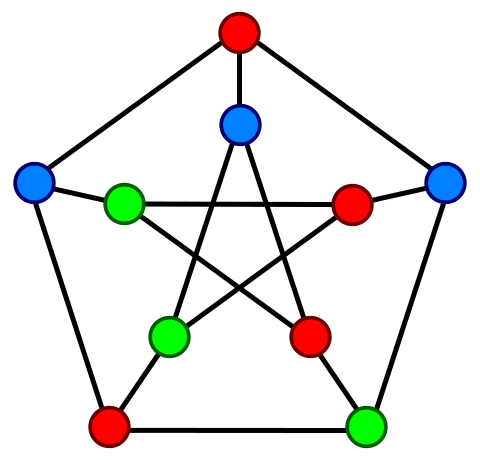
\includegraphics[width=0.4\textwidth]{Petersen_graph_coloring.png}
  \caption{Graph coloring of the Petersen's graph using three colors}
  \label{fig:petersen_coloring}
\end{figure}
In this section, we describe the syntax and semantics of \acrshort{fol},
for an extensive overview of \acrshort{fol}, we refer to \textcite{fo_overview}.

A formal language is a triple: \textit{vocabulary}, \textit{syntax} and \textit{semantics}. The vocabulary is the set of symbols that can be used. The syntax is the set of rules on how these symbols can be combined together. And the semantics is the way to interpret the statements. We omit the vocabulary, when it is clear from the context.

For each predicate $p$ and each function symbol $f$ in the vocabulary, we assume a natural number $n$ called \textit{arity} to be given, written as $p/n$ and $f/n$. This number indicates the number of parameters it takes; we often omit the arity when it is clear from the context. Propositional symbols are zero-arity predicates and constants are zero-arity functions. 
We assume propositional symbols \textit{true} and \textit{false}, whose domains are $\top$ and $\bot$ correspondingly, to be always in the vocabulary.

\begin{example}[Predicates and functions]\label{example:predicates_and_functions}
  Consider the famous problem of coloring a map, as in Figure \ref{fig:petersen_coloring}. The vocabulary would contain a predicate symbol \textit{border/2} and a function \textit{coloring/1}, together with a set of constants representing countries, such as \textit{belgium}, \textit{netherlands}, etc.
\end{example}

A \textit{structure} associates values with the predicates and functions from the vocabulary. A structure $I$ consists of

\begin{itemize}
  \item A domain $D^I$, which we also refer to as the \textit{universe}. The domain defines what are the possible values to be used.
  \item For each predicate $p/n$, the set of its values $p^I \subseteq \overbrace{D^I \times \dots \times D^I}^{n}$
  \item For each function symbol $f/n$,  $f^I$ the mapping  $\overbrace{D^I \times \dots \times D^I}^{n} \mapsto D^I$
\end{itemize}
We call the set of values $p^I$ for a predicate $p$  and the mapping $f^I$ for a function $f$ an \textit{interpretation}.

We assume the set of inequalities $\{ =, \neq, <, >, \leq, \geq \}$,  arithmetic $\{+, -, *, / \}$ and true $\top$, false $\bot$ to be interpreted by any interpretation in a standard way.

\begin{example}[Interpretaion of map coloring]
  Consider the predicate and the function from Example \ref{example:predicates_and_functions}. Then, $I$ can be the following:
  \begin{itemize}
    \item Domain $D^I = \{ \textit{red, green, blue, belgium, netherlands, germany, france} \}$
    \item The interpretation $\textit{border}^I = \{ (\textit{belgium, netherlands}), \dots \}$                                                                                     
    \item The interpretation $\textit{coloring}^I = \{ \textit{belgium} \mapsto \textit{green}, \dots \}$                                                                                     
  \end{itemize}
\end{example}


\paragraph{Syntax} 

The syntax of \acrlong{fol}, such as valid terms and formulae, is defined inductively.

A \textit{term} is defined as follows  
\begin{itemize}
  \item a \textit{variable} is a term
  \item if $t_1,\dots,t_n$ are terms and $f/n$ is a function, then $f(t_1,\dots,t_n)$ is term
\end{itemize}
We say a term $t$ is a \textit{domain term}, if $t$ is in the domain.


A \textit{formula} is defined as follows

\begin{itemize}
  \item if $p/n$ is a predicate and $t_1,\dots,t_n$ are terms, then $p(t_1,\dots,t_n)$ is a formula, called an \textit{atom}  
  \item if $\phi$ is a formula, then $\lnot \phi$ is a formula
  \item if $\phi$ is a formula and $x$ is a variable, then $\forall x: \phi$ and $\exists x: \phi$ are formulae 
  \item if $\phi$ and $\psi$ are formulae, then $\phi \wedge \psi$ and $\phi \vee \psi$ are formulae
\end{itemize}

We call a \textit{literal} an atom or the negation of an atom. An expression of the form $a \rightarrow b$ is a shorthand for $\lnot a \vee b$, and $a \leftrightarrow b$ is a shorthand for $a \rightarrow b \wedge b \rightarrow a$. A \textit{sentence} is a formula without free, i.e., non-quantified, variables. A set of sentences  is called a \textit{theory}.

\begin{example}[Formula]\label{example:formula}
  As in previous examples, we consider the problem of map coloring. The following formula:
  \begin{equation*}
    \forall X,Y{:}~\textit{border}(X,Y) \rightarrow \textit{coloring}(X) \neq \textit{coloring}(Y)
  \end{equation*}
has an indended meaning of enforcing the colours of adjacent countries to be different.
\end{example}


\paragraph{Semantics}
The semantics is defined inductively over the structure of the terms and of the formulae.

Let $I$ be a structure and $t$ be a domain term, then the \textit{value} of $t$ is $t^I = d$, where $d$ is the domain element. If $t$ is an expression of the form $f(t_1,\dots,t_n)$, then its value is $f^I(t_1^I,\dots,t_n^I)=d$, where $d$ is the domain element.

The truth assignment of a structure $I$ over formulae is defined inductively as follows:

\begin{itemize}
  \item $p(t_1,\dots,t_n)^I$ is true, iff $p^I(t_1^I,\dots,t_n^I)$ is true
  \item $(\lnot \phi)^I$ is true, iff $\phi^I$ is false
  \item $(\phi \wedge \psi)^I$ are true, iff $\phi^I$ and $\psi^I$ are true
  \item $(\phi \vee \psi)^I$ are true, iff $\phi^I$ or $\psi^I$ are true
  \item $\forall X: \phi$ is true, iff for each $d$ in $D^I$, $\phi[X/d]^I$ is true\footnote{$\phi[X/d]$ is a formula $\phi$, where each occurrence of $X$ is substituted with $d$}
  \item $\exists X: \phi$ is true, iff there is $d$ in $D^I$ such that $\phi[X/d]^I$ is true
\end{itemize}

We say that $I$ is a \textit{model} of or $I$ \textit{satisfies} a sentence $\phi$ iff $\phi^I$ is true, written as $I \models \phi$.

\begin{example}[Formula evalution]
  Assume, that the domain contains only two countries \textit{belgium} and \textit{netherlands} and two colors \textit{green} and \textit{red}. Let us show that $I$ with $\textit{border}$ being true for $(\textit{belgium,netherlands})$ and \textit{coloring} mapping \textit{belgium} to \textit{green} and \textit{netherlands} to \textit{red} is a model of the formula in Example \ref{example:formula}.

  \begin{tabular}{l l}
$(\forall X,Y{:}~\textit{border}(X,Y) \rightarrow \textit{coloring}(X) \neq \textit{coloring}(Y))^I$ & iff \\
for all $d_1,d_2 \in D$ holds $(\textit{border}(d_1,d_2))^I \rightarrow (\textit{coloring}(d_1) \neq \textit{coloring}(d_2))^I$ & iff \\
for $d_1 \neq \textit{belgium}$ and $d_2 \neq \textit{netherlands}$  the formula holds trivially & and if\\
for $d_1  = \textit{belgium}$ and $d_2 = \textit{netherlands}$,then $(\textit{belgium,netherlands})$ in $\textit{border}^I$ & and\\ 
      $f(\textit{belgium})^I = \textit{green} \neq \textit{red} = f(\textit{netherlands})^I$ holds & since \\
$\textit{green} \neq \textit{red}$  is true &
  \end{tabular}
\end{example}


\paragraph{Herbrand interpretation} The \textit{Herbrand Universe} is the set of all terms over the vocabulary without variables. A \textit{Herbrand Interpretaion} has the Herbrand Universe as its domain and interprets each symbol and function syntactically, e.g., a constant $a$ is interpreted by an interpretation $I$ as $a^I = a$. For any model that contains \acrlong{una} (\acrshort{una}) \parencite{UNA} and \acrlong{dca} (\acrshort{dca}) \parencite{DCA}, there exists an equivalent Herbrand model.


\section{Answer Set Programming}
\acrlong{asp} (\acrshort{asp}) is a logic programming paradigm for solving combinatorial and constraint optimization problems \parencite{whatisasp}.

Contrary to the programming language Prolog, which is based on a proof-theoretic approach to answer queries, ASP follows a model generation approach. It has been shown to be effective for a wide range of constraint satisfaction problems \parencite{ASPbook}.

The remainder of this section introduces the essentials of ASP in a rather informal way. ASP is a rich (and technical) research area, so we do not focus on technical issues as these would complicate the presentation, but rather refer the interested reader to \textcite{ASPbook,eiter,leone,whatisasp} for more details on this. For the actual implementation, we will use the Clasp system \parencite{ASPbook,BrewkaCACM}.

\begin{definition}[Disjunctive datalog program]
  A disjunctive datalog program is a finite set of rules of the form: 
  \begin{equation*}
    a_1 \vee a_2 \vee \dots \vee a_n \leftarrow b_1, \dots, b_k, \textit{ not }c_1,\dots,\textit{ not }c_h 
  \end{equation*}
\end{definition}
where $a_1, \dots, a_n, b_1, \dots, b_k,c_1, \dots c_h$ are atoms of a function-free First Order language $L$. Each atom is an expression of the form $p(t_1,\ldots,t_n)$, where $p$ is a predicate name and $t_i$ is either a constant or a variable. We refer to the head of rule $r$ as $H(r) = \{a_1,\dots,a_n\}$ and to the body as $B(r) = B^{+}(r) \cup B^{-}(r)$, where $B^{+}(r) = \{ b_1, \dots, b_k \}$ is the positive part of the body and $B^{-}(r) = \{ c_1, \dots, c_h \}$ the negative. 

If a disjunctive datalog program $P$ has variables, then its semantics are considered to be the same as that of its grounded version, written as \textit{ground(P)}, i.e. all variables are substituted with constants from the Herbrand Universe $H_P$ (the constants occurring in the program). The semantics of a program with variables is defined by the semantics of the corresponding grounded version.

\begin{example}
Let us demonstrate a simple example of an ASP program, it has four rules with variables and four facts, all predicates here are binary, except for \texttt{drive}, which is an unary predicate. The rule in Line 3 makes the connections undirected, while Lines 6 and 7 compute transitive closure of \texttt{road} predicate that are not blocked. The last route defines unary predicate \texttt{drive} as all cities reachable from \textit{berlin}.
    \begin{lstlisting}[caption=An example of an ASP program (from \textcite{ASPbook}); demonstrate possible route calculations for train connections around Berlin, label=lst:example_asp_program,basicstyle=\ttfamily]
road(berlin,potsdam).
road(potsdam,werder).
road(werder,brandenburg).
road(X,Y)  :- road(Y,X).
blocked(werder,brandenburg).
route(X,Y) :- road(X,Y), not blocked(X,Y).
route(X,Y) :- route(X,Z), route(Z,Y).
drive(X)   :- route(berlin ,X).
\end{lstlisting}
\end{example}

An interpretation $I$ w.r.t. to a program $P$ is a set of ground atoms of $P$. Let $P$ be a positive disjunctive datalog program (i.e. without negation), then an interpretation $I$ is called closed under $P$, if for every $r \in \textit{ground}(P)$ it holds that $H(r) \cap I \ne \emptyset$ whenever $B(r) \subseteq I$. 
\begin{definition}[Answer set of a positive program \parencite{eiter}]
An answer set of a positive program $P$ is a minimal (under set inclusion) interpretation among all interpretations that are closed under $P$.
\end{definition}

\begin{example}
An answer set of the program in Example \ref{lst:example_asp_program} would be the set: \{
\small
    \begin{tabular}{l l l}
    road(berlin,potsdam)     &road(potsdam,werder)   &road(werder,brandenburg) \\ 
    road(potsdam,berlin)     &road(werder,potsdam)   &road(brandenburg,werder)\\ 
    route(berlin,potsdam)    &route(potsdam,werder)  &route(brandenburg,werder)  \\
    route(werder,potsdam)    &route(potsdam,berlin)  &route(berlin,berlin) \\
    route(werder,berlin)     &route(potsdam,potsdam) &route(brandenburg,potsdam) \\
    route(berlin,werder)     &route(werder,werder)   &route(brandenburg,berlin) \\
    drive(potsdam)           &drive(berlin)          &drive(werder) \\
    blocked(werder,brandenburg) && 
\end{tabular}
\normalsize
 \}
\end{example}

Let us introduce the concept of a reduct \parencite{whatisasp}.
\begin{definition}[Gelfond-Lifschitz reduct] 
A reduct of a ground program $P$ w.r.t. an interpretation $I$, written as $P^I$, is  a positive ground program $P^I$ obtained by: 
\begin{itemize}
   \item removing all rules $r \in P$ for which $B^{-}(r) \cap I \ne \emptyset$;
   \item removing the literals ``$\textit{not }a$'' from all remaining rules.
 \end{itemize}
\end{definition}
Intuitively, the reduct of a program is a program where all rules with bodies contradicting $I$ are removed and in all non-contradicting all negative ones are ignored. The interpretation $I$ is a guess as to what is true and what is false.

\begin{definition}[An answer set of a disjunctive program]
An answer set of a disjunctive program $P$ is an interpretation $I$ such that $I$ is an answer set of positive ground program $\textit{ground}(P)^I$. 
\end{definition}

\begin{example} Consider the following disjunctive Datalog program $P$.
  \begin{eqnarray*}
    a \vee c  \leftarrow  b. \quad \quad b  \leftarrow  a, \textit{ not }c. \quad \quad a.
  \end{eqnarray*}
If we take the interpretation $I=\{a,b\}$ of $P$ as candidate answer set, then the reduct $P^I$ 
is  
\begin{eqnarray*}
    a \vee c \leftarrow b. \quad \quad   b \leftarrow a. \quad \quad  a.
\end{eqnarray*}
and it is easily seen that $I$ is a minimal interpretation closed under $P^I$, and therefore an answer set. 
\end{example}

We also use a special form of disjunctive rules called \textit{choice rules} \parencite{ASPbook}:
\begin{equation*}
  v_1~\{ a_1, a_2, \dots a_n \}~v_2 \leftarrow b_1, \dots, b_k, \textit{ not }c_1,\dots,\textit{ not }c_h
\end{equation*}
where $v_1$ and $v_2$ are integer constants. The semantics are as follows: if the body is satisfied, then the number of true atoms in $\{ a_1, a_2 \dots a_n \}$ is from $v_1$ to $v_2$.

An aggregate atom is an atom that has the following form: $l \# \{ a_1, \dots ,a_n \} u$
where $l$ and $u$ are constant numbers, each $a_i$ is a literal. The atom is true in an answer set $A$ iff there are from $l$ to $u$ literals $a_i$ that are true in $A$.

Another construct is \textit{maximization} \parencite{ASPbook, leone} (\textit{minimization} is defined analogously) stated as $\#\textit{maximize}\{ a_1=k_1, \dots, a_n=k_n \}$, 
where $a_1, \dots, a_n$ are classic literals and $k_1, \dots, k_n$ are integer constants (possibly negative). The semantics of this constraint are as follows: a model $I$ is selected if the weighted sum of $[a_i]*k_i$ is maximal in $I$, where $[\cdot]$ are Iverson brackets, i.e. $[a]$ is equal to $1$ iff $a$ is true in $I$ and $0$ otherwise.

\begin{example}
    \pubrev
    Let us demonstrate how the \textit{minimization} statement can be used in an ASP program. We use a standard problem of finding a Hamiltonian cycle, where the predicate \texttt{cost(X,Y,C)} is added and \texttt{C} represent the cost of picking a particular edge to be present in the cycle. Then the program not only finds a Hamiltonian cycle, but also minimizes its costs. In actual ASP encodings, we use \texttt{:-} for logical implication $\leftarrow$, as for the optimization statement a weight $C$ of an atom \texttt{cycle(X,Y)} is indicated as \texttt{cycle(X,Y) = C}.
\begin{minipage}{\linewidth}
    \begin{lstlisting}[caption=ASP encoding of the Hamiltonian cycle problem (due to \textcite{ASPbook}), label=lst:example_asp_coloring,basicstyle=\ttfamily]
1 { cycle(X,Y) : edge(X,Y) } 1 :- node(X). 
1 { cycle(X,Y) : edge(X,Y) } 1 :- node(Y).
reached(Y) :- cycle(a,Y).
reached(Y) :- cycle(X,Y), reached(X).
:- node(Y), not reached(Y).
#minimize [ cycle(X,Y) = C : cost(X,Y,C) ].
\end{lstlisting}
\end{minipage}
\pubrevend
\end{example}

We assume that arithmetic operators $\{ +, -, \times, / \}$ are present in the language and have the standard interpretation.

\begin{example}[Map Coloring in ASP]
  Let us demonstrate how the problem of map coloring discussed before can be expressed in ASP. 

  The first constraint ensures that the binary predicate \textit{coloring/2} is a function from nodes to colors and the second that if there are two nodes of the same color joined by an edge, then it is not a model.
\begin{lstlisting}[caption=ASP encoding of map coloring constraints, label=lst:example_asp_coloring,basicstyle=\ttfamily]
1 { coloring(X,C) : colors(C) } 1 :- node(X).

:- edge(X,Y), coloring(X,C), coloring(Y,C).
\end{lstlisting}
\end{example}

\paragraph{ASP systems: Clasp and Wasp}
In this thesis we make use of two existing ASP systems Clasp \parencite{clasp} and Wasp \parencite{wasp}. We mostly focus on the former and use the second to provide an experimental comparison on how two different system can execute the models with respect to runtime and memory usage.

Clasp extends the standard ASP theory described here with a number of features such as incremental grounding, preferences, satisfiability modulo theories, various solving parameters such as brave and cautious reasoning, parallel executions, heuristics and meta-programming \parencite{ASPbook}.

A typical modelling approach in ASP and in actual development with Clasp and Wasp follows guess and check paradigm. Where at first we define potential stable model candidates 
(typically through non-deterministic constructs) and then eliminate invalid candidates (typically through integrity constraints) \parencite{clasp, ASPbook, whatisasp}, which in a nutshell allows us to write the following formula for ASP modelling:

\begin{center}
    {\bfseries ASP Program = Data + Generator + Tester ( + Optimizer)} \footnote{\url{https://www.cs.uni-potsdam.de/~torsten/potassco/slides/asp.pdf}}
\end{center}

We follow this modelling paradigm throughout the thesis. To demonstrate it, consider as an example, $n$-queen modelling problem, where one needs to put a number of queens on the board such that no queen attacks another. This can be modelled as in Listing \ref{lst:n_queens_example_modelling}. first we specify data as facts, in Lines \ref{background:line:data1} and \ref{background:line:data2}, then we define the set of possible answer sets using a choice rule in Line \ref{background:line:choice} and finally we validate them in Lines \ref{background:line:int1},\ref{background:line:int2} and \ref{background:line:int3}. 
\pubrev
In greater detail, we require the number of queens to equal to $k$ by using a cardinality constraint in Line \ref{background:line:choice} then right after this ''guess`` is verified with integrity constraints: no queen is no the same row (Line \ref{background:line:int1}), no queen in the same column (Line \ref{background:line:int2}) or the same diagonal (Line \ref{background:line:int3}). An answer set that has a set of $k$ queens which satisfy the integrity constraints is therefore a solution to $k$-queen problem.
\pubrevend

\begin{figure}[H] 
\renewcommand\figurename{Listing}
\begin{Verbatim}[fontsize=\small,numbers=left,xleftmargin=0mm,commandchars=\\\{\},frame=single]
% Data specifying the board
col(1..k).\label{background:line:data1}
row(1..k).\label{background:line:data2}
% Choice rule to specify possible stable models
k \{ queen(Row,Col) : col(Col), row(Row) \} k. \label{background:line:choice}
% Integrity constraint to validate the candidate models
:- queen(Rw,Cw), queen(Rb,Cb), Rw  = Rb, Cw != Cb. \label{background:line:int1}
:- queen(Rw,Cw), queen(Rb,Cb), Rw != Rb, Cw  = Cb. \label{background:line:int2}
:- queen(Rw,Cw), queen(Rb,Cb), Rw != Rb, | Rw - Rb | = | Cw - Cb |.\label{background:line:int3}
\end{Verbatim}
\caption{An ASP guess-and-check paradigm modelling example on the $n$-queen problem}
\label{lst:n_queens_example_modelling}
\end{figure}


\section{Constraint programming}
A detailed introduction to \acrlong{cp}(\acrshort{cp}) can be found in the ''Handbook of Constraint Programming`` \parencite{handbookcp}. A basic concept here is that of a variable $v$ which always has an associated domain $d$, a domain here is simply a set of constants. An example domain is the Boolean domain \{ True, False \}. A constraint $c$ is an expression of the form \textit{name(vars)}, where \textit{vars} is a list of variable names and \textit{name} is the type of constraints from a predefined set of constraint classes. Examples of classes of constraints are comparisons,   arithmetic operations, list and set constraints (all-different, permutations, etc). We denote the set of all variables as $V$, of all domains as $D$ and of constraints as $C$, then a triple $(V,D,C)$ is a constraint programming model and a \acrlong{csp} (\acrshort{csp}) is the problem of finding an assignment $A$ for $V$ over $D$ satisfying all constraints $C$.

Let us demonstrate how it is possible to model the map coloring problem in MiniZinc\footnote{MiniZinc is popular constraint programming language \url{http://www.minizinc.org/}. Based on the encoding from \url{www.hakank.org/minizinc/map.mzn}.}  
\begin{lstlisting}
% number of countries
int: n; 
% [belgium,denmark,france,germany,netherlands,luxembourg]
array[1..n] of var 1..4: country; 
% the map (as a binary matrix)
array[1..n,1..n] of 0..1: connections; 

forall(i,j in 1..n where i < j /\ conn[i,j] = 1) (
              country[i] != country[j]
      )
\end{lstlisting}
The first lines define variables together with their types, for example \texttt{country} is an array, each element of which can take value from one to four. And the constraint at the bottom of the listing verifies that for each value of indices $i,j$ in the range of 1 to n such that (part: \texttt{where}) $i$ is smaller than $j$ (part: \texttt{i < j}) and there is a connection between $i$ and $j$ (part: \texttt{conn[i,j] = 1}) it holds that colors of the countries are different, i.e., the part: \texttt{country[i] != country[j]}.

Let us introduce the key definitions from constraints programming formally.
\begin{definition}[\acrlong{csp}(\acrshort{csp})]
    A \acrshort{csp} is a triple $(V,D,C)$ where
    \begin{itemize}
        \item $V$ is a finite set of variables (a set of distinct symbols)
        \item $D$ is a domain that maps every variable $v$ in $V$ to a set of its possible values $D_v$ (a set of district symbols, disjoint from the variable symbols)
        \item $C$ is a finite set of constraints (language dependent)
    \end{itemize}
\end{definition}

A solution $A$ is a mapping function from $V$ to $D$ such that for every constraint it holds that for every constraint $c$ in $C$, the constraint $c^A$, which is the constraint $c$ where each variable $v$ is replaced with $A(v)$, holds.

\pubrev 
In case of the problem above,  \texttt{n} is the constant that represents the number of countries, \texttt{conn[i,j]} represents the fixed connections between countries (is there or not) and each \texttt{country} represent an array of variables that can get assigned a colour, each country gets a colour. The domain is essentially specifying that \texttt{conn[i,j]} can be either one or zero and \texttt{country[i]} can be mapped to a color value (and the list of colours itself is restricted by the domain itself), which is represented as a number from 1 to 4 here. Assuming that for example there is only one connection \texttt{conn[1,2]} and two countries one and two, then solution assignment $A$ maps \texttt{country[1]} to one and \texttt{country[2]} to two (connection \texttt{conn[1,2]} is indeed also mapped to one as the given data).
\pubrevend

A constraint optimization problem is a \acrshort{csp} $(V,D,C)$ extended with an objective function $f_o$ from $V$ to $R^1$, then the problem is to find a solution to the original \acrshort{csp} such that the score defined by $f_o$ is maximal (or minimal).

A typical approach to solving a constraint satisfaction problem is to use a form of search over the variable values in their domains, we present here an overview over a possible searching procedure, for details we refer to \textcite{tias_phd}.

Algorithm \ref{algo:simple_search} demonstrates how we can solve a \acrshort{csp}. First, we propagate all possible deterministic assignments. Then we make a decision which variable we are going to split, i.e., we investigate two cases separately when it can take certain values and when it cannot. For each of this cases we call the procedure itself recursively. If in certain moment, we have derived that all variables have only one value, then it is a solution, if in certain point of propagating values using given constraints we established that no value is left for a variable, we return a failure for this particular case.

\begin{algorithm}[t]
    \begin{algorithmic}[1]
        \footnotesize
        \State $D \gets \textit{propagate}(D)$ \label{line:propagate}
        \If{ $\exists v: D_v = \emptyset$} \label{line:back}
        \State \Return $\bot$
        \EndIf
        \If{$\exists v \in V: |D_v| > 1$}
        \State $v = \textit{select\_variable}(V)$ \Comment{pick the most promising variable}
        \State $D_s = \textit{split}(D_v)$  \Comment{$D_v$ is the domain of $v$}
        \State $\texttt{search}(D \cup \{ v \mapsto D_s \})$ \Comment{recursive DFS-like search}
        \State $\texttt{search}(D \cup \{ v \mapsto D_v / D_s \})$
        \Else
        \State \Return \textit{assignment}
        \EndIf
    \end{algorithmic}
    \caption{Simple constraint propagate-and-search algorithm: search(D)}
    \label{algo:simple_search}
\end{algorithm}

\pubrev
Let us elaborate on both key steps of the Algorithm \ref{algo:simple_search}.
\paragraph{Search} Many popular CP frameworks follow the Deep First Search (DFS) strategy as described in the presented algorithm \parencite{cp_propagation,handbookcp}. Other techniques exist as well \parencite{other_search_CP} but we focus only the most popular DFS approach described here.

For a constraint satisfaction problem, its search tree represents an order from more general to more specific domains. The tree root has its original the most general (yet unrestricted) domain. The leaves of a search tree represent actual solutions to the given \acrshort{csp}: each $v \in V$ is mapped to a single value $d$ from $D_v$. Each node represents branching of the search by domain splitting. If a constraint is violated, then Line \ref{line:back} starts the backtracking mechanism (DFS is a form of backtracking search).

\paragraph{Propagation} is a search speed up mechanism. In Algorithm \ref{algo:simple_search} it appears in Line \ref{line:propagate}. The key idea behind this mechanism is in the domain reduction and so called, \textit{local consistency}, i.e., satisfaction or actually violation of a subset (even a single one) constraints. This removes values that definitely cannot be in the solution since they violate one or more constraints. Contrary, \textit{global consistency} ensures that all constraints in the model are satisfied. The latter is indeed hard to achieve, the former is easy to check, since you can check one or several constraints in the isolation, or in the other words, locally. If a certain value violates this constraint, then it definitely cannot be in the solution set. Many various methods to check local consistency exist \parencite{cp_christian_local_consistency}: node consistency, arc consistency and path consistency, etc.

To keep local consistency for constraints, \textit{propagation rules} and \textit{propagators} are applied. Such a rule, takes an original domain $D$ \sergey{finish}

\pubrevend
\section{\fod and the IDP System}
The knowledge based language \fod is the extension of First Order Logic with a number of features, such as, inductive definitions and aggregates. The IDP system \parencite{idppaper} is the reasoning system that accepts as input the \fod language and is able to perform a number of reasoning tasks: such as finding logical models, model checking and theorem proving. IDP and its language FO(.) can be seen as executable logic we have discussed before in Section \ref{sec:fol}. 

Let us illustrate an inductive definition and an IDP program by example, see Listing \ref{lst:idp_reachability}, where Reach(x,y) is an example of an inductive definition, defined via the base case and the inductive step (see the Theory part).
\begin{lstlisting}[caption=An example of an inductive definition in FO(.) and of an IDP program,label=lst:idp_reachability]
vocabulary V{
  type Node
  Edge(Node, Node)
  Reach(Node, Node)
}

theory T:V{
  { 
    Reach(x,y) <-      Edge(x,y).
    Reach(x,y) <- ?z : Edge(x,z) & Reach(z,y).
  }
}

structure S:V{
  Node = {1;2;3}
  Edge = {1,2; 2,3; 3,1} 
}
\end{lstlisting}

An IDP program has three parts: \textit{Vocabulary} that defines the terminology and concepts of a problem, \textit{Structure} that sets certain values to true or false, and \textit{Theory} introduces constraints.

For example the sushi problem can be encoded in IDP as in Listing \ref{lst:idp_sushi}. First, we define vocabulary, which corresponds to vocabulary in first order logic, except for the extra type information. Facts and domains are specified in the structure section, as we see for example with the declaration of the domain for the type person, for which actual values are assigned in the section structure. The theory section defines the actual clauses or constraints, which indeed corresponds to the first order sentences, the only constraint here one to one maps to Eq. \ref{eq:sushi}, which a classical logical implication. The procedure \texttt{main} is a directive to the system to extend the given structure satisfying the constraints in the theory.

\begin{minipage}{\linewidth}
\begin{lstlisting}[caption=Encoding sushi preferences problem, label=lst:idp_sushi,basicstyle=\ttfamily, basicstyle=\small]
vocabulary V{
  type person
  allergic(person)
  vegan(person)
  likes_sushi(person)
}
theory T:V{
  !x[person]: ~allergic(x) & ~vegan(x) => likes_sushi(x).
}

structure S:V{
  person   = {peter; alina; ronald}
  vegan    = {ronald}
  allergic = {peter}
}

procedure main(){
  M = modelexpand(T,S)[1]
  print(M)
}
\end{lstlisting}
\end{minipage}

Therefore, when we write a first order model for a problem, we can always map it to the language of FO(.), furthermore provided language extensions make modelling of relational problems more natural and convenient.

\pubrev
FO(.) and the system implementing it, IDP, can be seen a form of constraint logic programming. Where one models a problem using a set of constraints expressed as logical formulae. 
Let us demonstrate this on an example. 
\begin{example}[Constrained Pizza Selection Problem]\label{example:pizza}
	Peter, Alina, Ronald and Sergey decided to order three pizzas in a trattoria: margarita, veggie and meat-lovers -- each pizza can be shared by at most two people and everyone specified pizzas they can eat, together with their preferences for the selected pizzas on the scale from one to ten. Can we help them to share the pizzas in an optimal way?

    We start with modelling the domain of the problem, there are four \textit{persons}, which is captured by a type declaration, \texttt{type person}, in the same way we capture the domain of available \textit{pizzas}, see first lines of \texttt{Vocabulary} in Listing \ref{lst:pizza_selection}. Then, once these two types are declared, in \texttt{Structure} we assign actual values to them, like
\begin{verbatim}
pizza  = {margaritha; veggie; meat}
\end{verbatim}
    IDP interprets this as the truth assignment, only specified constants belong to the type \texttt{pizza} and nothing else. Similarly, we define who can eat what pizza, e.g., Alina can eat veggie pizza and meat-lovers pizza, we see that clearly it's a binary relation between a \texttt{person} and a \texttt{pizza}, then we declare it as \texttt{can\_eat(person,pizza)} and its actual domain as 
\begin{verbatim}
can_eat = {
          (alina,veggie); (alina,meat); 
          (sergey,margaritha); (sergey,meat);
          (ronald,margaritha); (ronald,veggie);
          (peter,meat)
          }
\end{verbatim}
which specifies all legitimate pairs of \textit{(person,pizza)} to be used.

    
To specify preferences over the selection, we introduce the partial function \texttt{partial preferences(person,pizza):score} (and the type \texttt{score} which is a subtype of integers) as the following mapping:
\begin{verbatim}
ronald,veggie -> 10;    ronald,margaritha -> 1; 
alina,veggie  -> 5;     alina,meat  -> 7;
sergey,margaritha -> 2; sergey,meat -> 7;
peter,meat -> 10
\end{verbatim}
\end{example}
First, we use a partial function because we already know we should only define this function on the pairs specified in \texttt{can\_eat}. Second, we introduce score because we know exactly the range of values it takes and therefore helps the IDP solver to look for a solution more efficiently.

Now we need to define what we are looking for: the binary predicate \texttt{eats(person,pizza)}. This predicate determines who eats what and based on it, we are going to compute the overall \textit{satisfaction} score. Simply speaking, what we are looking for is the best values (in terms of preferences) for \texttt{eats} that satisfy all specified constraints (on sharing pizzas, etc).

What are the constraints and how do we model them? First, we know that each person eats a pizza and each pizza is eaten by a person. These are constraints of the form: for each A there is a B,
\begin{verbatim}
// each person eats a pizza 
!s[person]: ?p[pizza]: can_eat(s,p) & eats(s,p). 
\end{verbatim}
Since IDP supports types, this is essentially a direct formalization of: for each person, there must exist a pizza such that this person can eat this pizza and he eats it. Similarly, we formulate it for pizzas. The no-sharing constraint is modelled in a bit of different manner: we say that if two people eat a pizza, there cannot be a third person that is different from these two (see \texttt{Theory} in Listing \ref{lst:pizza_selection}).

Then, to obtain \textit{an optimal} solution, we introduce an optimization statement:
\begin{verbatim}
term O:V{
 sum{prsn[person],pzz[pizza],score[score]: 
 eats(prsn,pzz) & preferences(prsn,pzz)=score:score}
}
\end{verbatim}
what it does is the following: it sums all preference scores for all pairs of person and pizza \texttt{(prsn,pzz)} that the binary predicate \texttt{eats} assigns to true, or simply speaking, it sums scores corresponding to the assigned values in \texttt{eats}, which gives to us a measure of quality of a found model. Then we ask the IDP system to find a model that maximizes this measure.

Let us demonstrate the full model solving this program in Listing \ref{lst:pizza_selection}.
\begin{minipage}{\linewidth}
\begin{lstlisting}[caption=Encoding pizza selection problem, label=lst:pizza_selection,basicstyle=\ttfamily, basicstyle=\small]
vocabulary V{
 type person
 type pizza
 can_eat(person,pizza)
 eats(person,pizza)
 type score isa int
 partial preferences(person,pizza): score
}
theory T:V{
 !s[person]: ?p[pizza]: can_eat(s,p) & eats(s,p). // each person eats a pizza 
 !p[pizza]: ?s[person]: can_eat(s,p) & eats(s,p). // each pizza is eaten by someone
 // no pizza is share by more than 2 people
 !person1[person], person2[person], p[pizza]: person1 ~= person2 & eats(person1,p) & eats(person2,p) => ~?person3[person]: eats(person3,p) & person1 ~= person3 & person2 ~= person3.
}

structure S:V{
 person = {peter; alina; ronald; sergey}
 pizza  = {margaritha; veggie; meat}
 score  = {1..10}
 can_eat   = {
        	(alina,veggie); (alina,meat); 
         	(sergey,margaritha); (sergey,meat);
         	(ronald,margaritha); (ronald,veggie);
         	(peter,meat)
     	 }
 preferences = {	
            ronald,veggie -> 10; ronald,margaritha -> 1; 
            alina,veggie  -> 5;  alina,meat-> 7;
            sergey,margaritha ->2 ; sergey,meat->7;
            peter,meat -> 10
        	   }	
}
// we maximize overall preferences
term O:V{
    sum{prsn[person],pzz[pizza],score[score]: 
    eats(prsn,pzz) & preferences(prsn,pzz)=score:score}
}

procedure main(){
    result = maximize(T,S,O)[1]
    print(result)
}

\end{lstlisting}
\end{minipage}
\pubrevend


\pubrev
   \section{Relational pattern mining}
   The task of relational pattern mining is to mine queries in a logical and relational learning setting. Starting with the work the Warmr system \parencite{warmr}, there has been a line of work that focusses on the following frequent query mining problem \parencite{bagm,farmer,condensed_luc}:

   \noindent
   {\bf Given:} \vspace{-8pt}
   \begin{itemize}
   \item a relational database $D$,
   \item the entity of interest determining the \keypred/1 predicate,
   \item a frequency threshold $t$,
   \item a language ${\cal L}$ of logical queries of the form $\keypred(X) \leftarrow b_1, ..., b_n$ defining $key/1$ ($b_i$'s are atoms).
   \end{itemize}\vspace{-5pt}
   {\bf Find:} all queries $c \in {\cal L}$ s.t. $\freqpred(c,D) \geq t$, where ${\freqpred(c,D) = |\{\theta \mid D \cup c \models key(X)\theta \}|}$.

   Notice that the substitutions $\theta$ only substitute variables $X$ that occur in \keypred. 

   Here we focus our attention on graph data, as this forms the simplest truly relational learning setting and allows us to focus on what is essential for extending the declarative modelling paradigm to a relational setting. 
    
   As an example, consider a graph database $D$, represented by the facts 
   \begin{equation*}
   \{ \edge(g_1,1,2),~ \edge(g_1,2,3),~ \edge(g_1,1,3),~ \edge(g_2,1,2),~ \edge(g_2,2,3), \dots \},
   \end{equation*}
   where the ternary relation $\edge(g,e_1,e_2)$ states that in graph $g$ there is an edge between $e_1$ and $e_2$ (we assume graphs to be undirected, so there is also always an edge between $e_2$ and $e_1$). The frequency of $\textit{key}(K) \leftarrow \edge(K,B,C), \edge(K,C,D), \edge(K,B,D)$ in this database is 2 as the query returns $g_1$ and $g_2$. If $key(g)$ holds,  then the graph $g$ is subsumed by the query specified defined in the body of the clause for \keypred.
   In this section we briefly recap the necessary background both from the field of pattern mining.

   Let $\mi{D}$ be a dataset, $\patternspace$ a language for expressing pattern properties or defining subgroups of the
   data, and $\mi{q}$ a selection predicate. %Then t
   The task of pattern mining is to find $\mi{Th}(\patternspace,D, \mi{q})= \{\phi \in \patternspace\, |\, \mi{q}(D, \phi) \text{ is true}\}$ (see the seminal work by \cite{DBLP:journals/datamine/MannilaT97}). 

   Pattern mining has been mainly studied for % in three settings: 
   itemsets, sequences, graphs and queries. These settings are determined by the language of $\patternspace$. 
\pubrevend
